\section{HSV}
Nella strutturazione del progetto ci è venuto molto naturale andare a lavorare con una scala di colori HSV.

Ma perchè non applicare un filtraggio basato su RGB?

Come noto nella letteratura, nell'ambito dell'\textit{image recognition} è usuale il problema di andare a mascherare un colore piuttosto che un altro, come nel nostro caso.

Potremmo voler trovare, sempre per esempio, oggetti di colore rosso, scannerizzando nell'immagine solamente colori (255,0,0) nella scala RGB: con questo approccio andremmo ad applicare una condizione troppo stringente ai colori.
Si potrebbe pensare, come soluzione a questa condizione parecchio stringente, di trovare colori in un range di rossi, come per esempio {(130,0,0);(255,0,0)}: il problema comunque persisterebbe proprio per il fatto che il rosso è ottenuto come combinazione di più colori primari, e non come un solo singolo colore.

Potremmo pensare dunque, di andare a fondo del problema,cambiando gli intervalli dei valori RGB per tutti i colori primari ma sarebbe uno sforzo non secondario e probabilmente con risultati poco significativi.
È necessario un metodo che abbia meno parametri per semplificare l'identificazione dei colori: questo metodo è rappresentato proprio dall'utilizzo del HSV.

\begin{figure}[H]
	\centering
	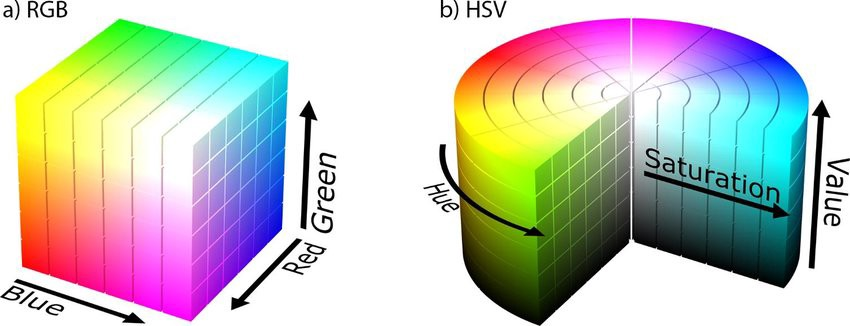
\includegraphics[width=0.5\textwidth]{Immagini/HSV_RGB.jpeg}
	\caption{RGB vs HSV}
	\label{fig:RGB_&_HSV}
\end{figure}

Si può notare come, in Fig \ref{fig:RGB_&_HSV}, il colore rosso sia definito in un range ben chiaro di un solo valore (\textit{Hue}) mentre \textit{Saturation }and \textit{Value} servono solo a limitare ulteriormente la gamma di tonalità di rosso accettabili. 

\section{Frecce o cerchi?}
Nel progetto utilizzato come punto di partenza, si erano individuati cerchi di diversa grandezza per testare le funzionalità della libreria OpenCV nell' object detection.

Ovviamente l'utilizzo di cerchi limita di molto l'espressività del simbolo in quanto un cerchio non può, per sua natura identificare una direzione, men che meno un verso.
Le frecce sono quindi la soluzione più naturale al problema di identificare con un simbolo una direzione ed un verso che poi, un eventuale robot mobile, potrà seguire.

TODO mettere foto cerchi e frecce
foto maschera

\section{Maschere}
Le maschere sono fondamentali nel processo di object detection tramite la libreria OpenCV.

Queste ultime sono immagini binarie (bianco e nero) e sono utilizzate da tutte le funzioni di identificazione dei contorni e interpolazione di punti presenti in OpenCV.
La seguente linea di codice

\begin{lstlisting}
	inRange(original_image_hsv, Scalar(MinH_R, MinS_R, MinV_R), Scalar(MaxH_R, MaxS_R, MaxV_R), hsv_red);
\end{lstlisting}

permette di identificare tutti gli oggetti di colore rosso e di salvarli nella Matrice \textit{hsv\_red}.

\section{Erosione e dilatazione}
L'erosione e la dilatazione sono tecniche note allo stato dell'arte attuale utili per rimuovere rumore da una immagine.

\begin{figure}[H]
	\centering
	
\includegraphics[width=0.5\textwidth]{Immagini/erosion_dil.png}
	\caption{Erosione e dilatazione}
	\label{fig:erosion_dil}
\end{figure}

Nel caso preso in considerazione da questo report è stato necessario applicare la tecnica di erosione solamente alla parte inferiore dell'immagine in quanto, se applicata nella parte superiore, avrebbe eliminato oltre al rumore anche un'eventuale freccia che sarebbe apparsa molto piccola.

Da sottolineare è il fatto che la tecnica di erosione e successiva dilatazione è stata applicata solamente alle figure rettangolari rosse in quanto la funzione di dilatazione prevede un kernel per la computazione del filtro: dato un kernel definito da una x e una y risulterebbe quanto mai complesso effettuare una dilatazione che rassomigli poi ad una forma triangolare.